\providecommand{\pgfsyspdfmark}[3]{}
\providecommand{\savepicturepage}[3]{}

\documentclass[11pt,letterpaper]{article}
\usepackage[lmargin=1in,rmargin=1in,tmargin=1in,bmargin=1in]{geometry}

% -------------------
% Packages
% -------------------
\usepackage{
	amsmath,			% Math Environments
	amssymb,			% Extended Symbols
	enumerate,		    % Enumerate Environments
	graphicx,			% Include Images
	lastpage,			% Reference Lastpage
	multicol,			% Use Multi-columns
	multirow,			% Use Multi-rows
	gensymb
}


% -------------------
% Font
% -------------------
\usepackage[T1]{fontenc}
\usepackage{charter}
\usepackage{tasks}


% -------------------
% Commands
% -------------------

\newcommand{\prob}{\noindent\textbf{Problem. }}
\newcounter{problem}
\newcommand{\problem}{
	\stepcounter{problem}%
	\noindent \textbf{Problem \theproblem. }%
}
\newcommand{\pspace}{\par\vspace{\baselineskip}}
\newcommand{\ds}{\displaystyle}


% -------------------
% Header & Footer
% -------------------
\usepackage{fancyhdr}

\fancypagestyle{pages}{
	%Headers
	\fancyhead[L]{}
	\fancyhead[C]{}
	\fancyhead[R]{}
\renewcommand{\headrulewidth}{0pt}
	%Footers
	\fancyfoot[L]{}
	\fancyfoot[C]{}
	\fancyfoot[R]{}
\renewcommand{\footrulewidth}{0.0pt}
}
\headheight=0pt
\footskip=14pt

\pagestyle{pages}


% -------------------
% Content
% -------------------
\begin{document}
\noindent\textbf{\large Calculus II (MSF\_10010 / AM\_\_1080AH) \\ 2023 Spring \\ Problem List XIII (Due June 1)}

\bigskip

\problem Find the following partial derivatives:
\begin{tasks}(3)
	\task $\frac{\partial}{\partial x} (x^3 + 3x^2y + 3xy^2 + y^3)$
	\task $\frac{\partial}{\partial y} [(x + y^2)e^y]$
	\task $\frac{\partial}{\partial t} [x \sqrt[y]{y} + \sin(x^{y^2+4x})]$
	\task $\frac{\partial^2}{\partial x^2} \sqrt{x^2 + 4xy}$
	\task $\frac{\partial^2}{\partial x \partial y} [x\ln(3x + 2y)]$
\end{tasks}

\vspace{6mm}

\problem Find all the critical points for the following function of two variables:
\[f(x, y) = \sqrt{x^2+y^2} - \frac{x^2 + 8y}{10}\]
(Hint: There are two critical points)
\vspace{6mm}

\problem Find all local minima of $f(x,y) = x^3 + 3xy + y^2$ using partial derivatives.  Verify that your answers are local minima with the second partial derivative test.

\vspace{6mm}

\problem In class, we heuristically argued that given a function $f(x,y)$ and a point $(x_0, y_0)$ that satisfies $f_x(x_0, y_0) = f_y(x_0, y_0) = 0$, the signs of $f_{xx}(x_0,y_0)$ and $f_{yy}(x_0,y_0)$ are not sufficient to argue if $f$ attains local extremum at $(x_0, y_0)$.  Here we will demonstrate with the function $f(x, y) = x^2 - 6xy + y^2$ and the point $(0,0)$.
\begin{enumerate}[a)]
	\item Show that $f_x(0,0) = f_y(0,0) = 0$.  This implies that $f$ is locally flat around $(0,0)$.
	\item Calcultate $f_{xx}(0,0)$.  Based on the result, is the trace of $z = f(x,y)$ on $y=0$ (the $xz$ plane) concave up, concave down or neither at $x = 0$?
	\item Calcultate $f_{yy}(0,0)$.  Based on the result, is the trace of $z = f(x,y)$ on $x=0$ (the $yz$ plane) concave up, concave down or neither at $y = 0$?
	\item As shown in the figure, we can rotate the $xy$-axes counter-clockwise by $45\degree$ to arrive at the $uv$-axes.  The relationalship between the original coordinate $(x,y)$ and new coordinate $(u,v)$ will then be $x = \frac{u-v}{\sqrt{2}}, y = \frac{u+v}{\sqrt{2}}$.  Substitute $x, y$ with $u, v$ in $f(x,y)$ to obatain a new function $\Tilde{f}(u,v)$.
	\item Calcultate $\Tilde{f}_{uu}(0,0)$.  Based on the result, is the trace of $z = \Tilde{f}(u,v)$ on $v=0$ (the $uz$ plane) concave up, concave down or neither at $u = 0$?
	\item You should see that the concavity of the traces at $(0,0)$ are different between the direction of $x$-axis (or $y$-axis) and $u$-axis, which implies that $(0,0)$ is a saddle point.  Verify this by calculating the discriminant $D$ at $(0,0)$.
\end{enumerate}

\begin{center}
    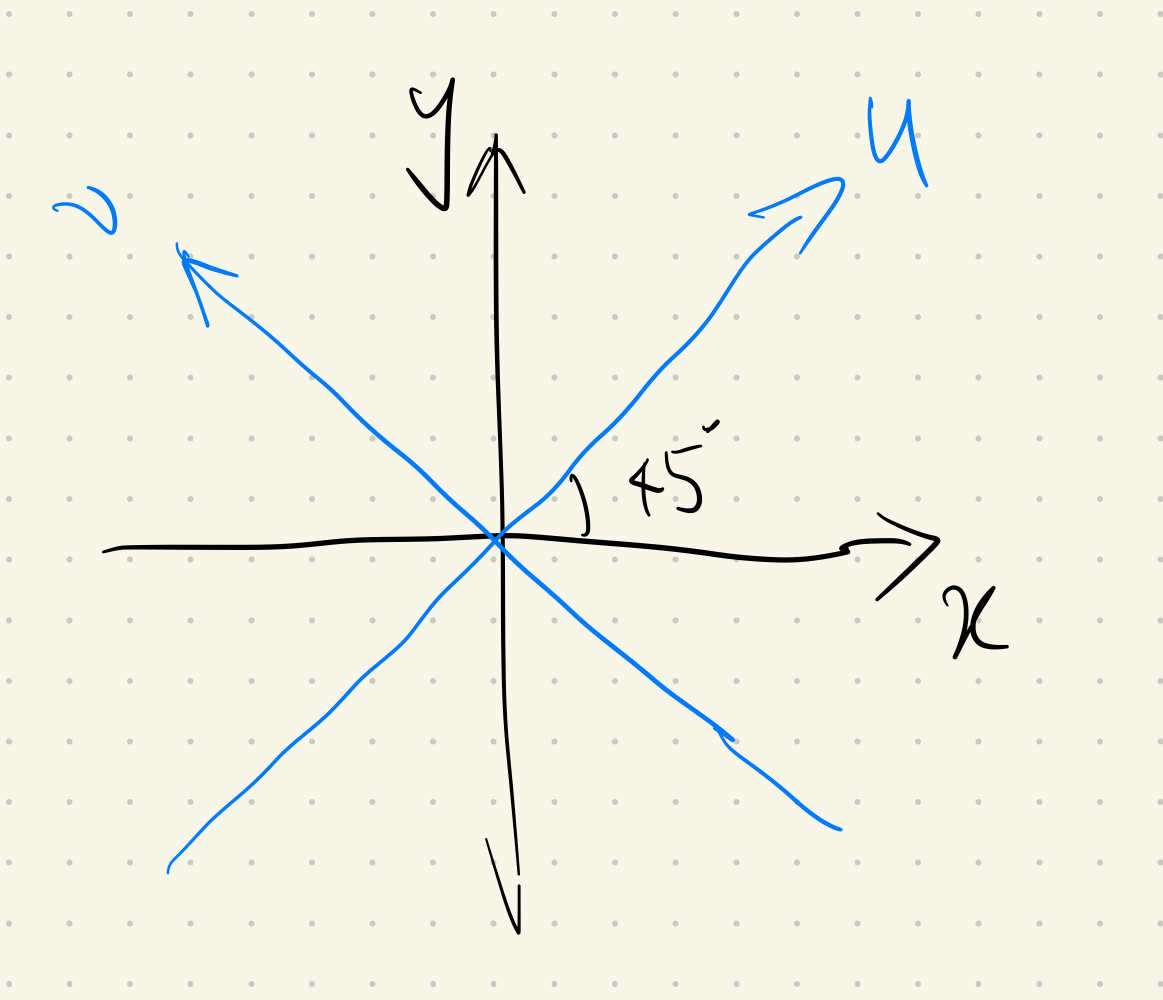
\includegraphics[width = 0.3\textwidth]{../graph/A13.png}
\end{center}

\end{document}